\documentclass[border=10pt]{standalone}
\usepackage[svgnames]{xcolor}
\usepackage{amsmath}
\usepackage{pgfplots}
\pgfplotsset{compat=newest}
\usepackage[sfdefault]{FiraSans}
\usepackage{FiraMono}
\renewcommand*\familydefault{\sfdefault}
\begin{document}
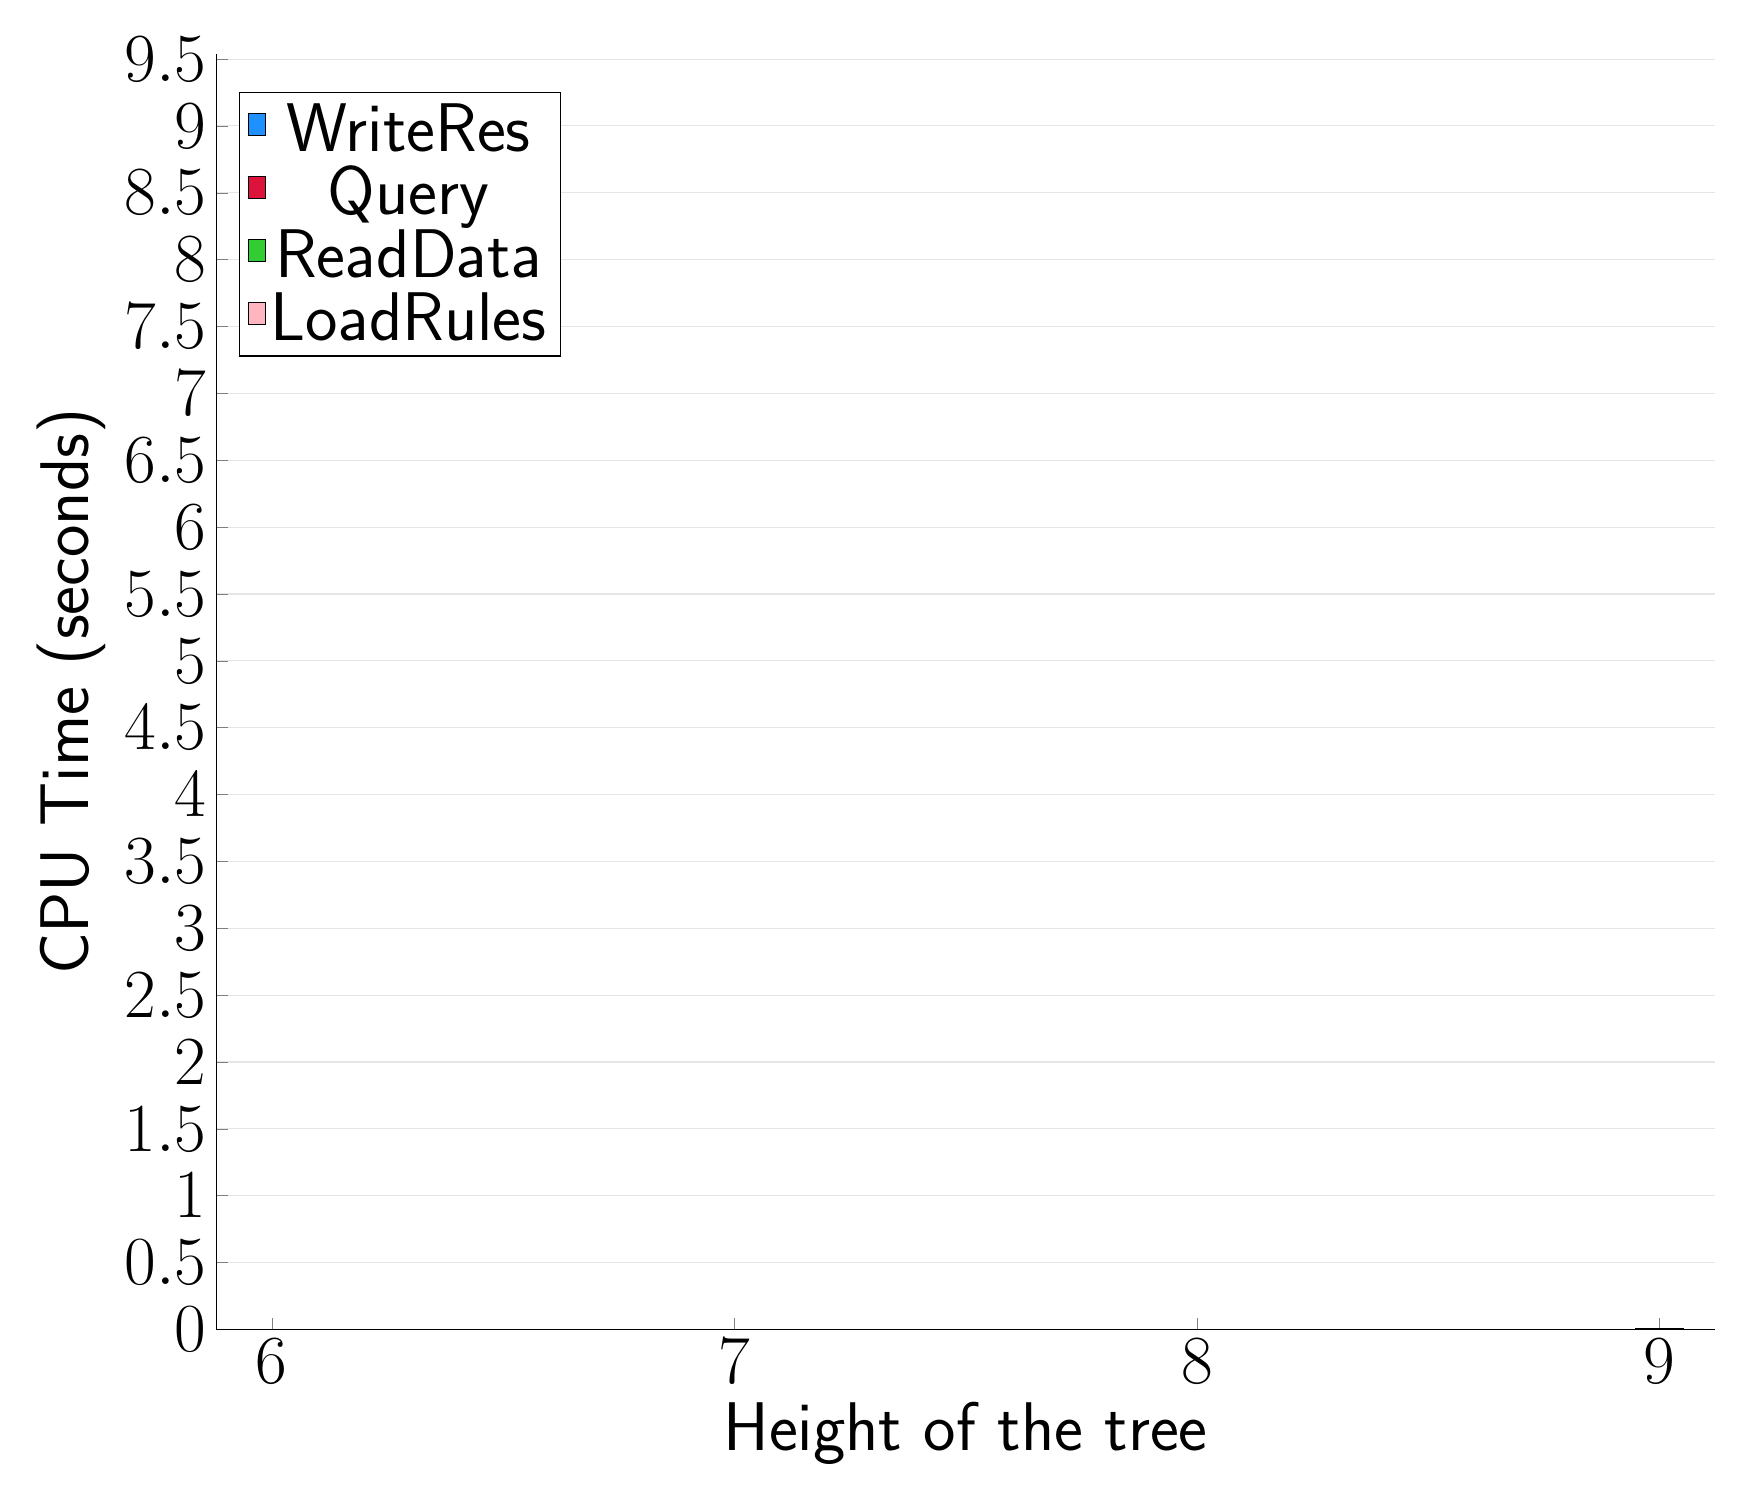
\begin{tikzpicture}
\begin{axis}[
   ybar stacked,
   width=1.7\textwidth,
   bar width=0.6cm,
   ymajorgrids, tick align=inside,
   major grid style={draw=gray!20},
   xtick=data,
   ymin=0, ymax=9.538,
   axis x line*=bottom,
   axis y line*=left,
   enlarge x limits=0.04,
   legend style={
       at={(0.23, 0.97)},
       anchor=north east,
       legend columns=1,
       font=\Huge,
   },
   ylabel={CPU Time (seconds)},
   xlabel={Height of the tree},
   label style={font=\Huge},
   tick label style={font=\Huge},
]
\addlegendimage{fill=DodgerBlue, draw=black, line width=0.2pt}
\addlegendentry{WriteRes}
\addlegendimage{fill=Crimson, draw=black, line width=0.2pt}
\addlegendentry{Query}
\addlegendimage{fill=LimeGreen, draw=black, line width=0.2pt}
\addlegendentry{ReadData}
\addlegendimage{fill=LightPink, draw=black, line width=0.2pt}
\addlegendentry{LoadRules}
\addplot +[fill=LightPink, draw=black, line width=0.55pt] coordinates {
(6, 0.0005588000000000002)
(7, 0.000552)
(8, 0.0005522000000000002)
(8, 0.0005519999999999996)
(8, 0.0005528000000000002)
(9, 0.0005499999999999995)
(9, 0.0005534000000000004)
(9, 0.0005574)
(9, 0.0005586000000000005)
(9, 0.0005596)
};
\addplot +[fill=LimeGreen, draw=black, line width=0.55pt] coordinates {
(6, 0.00017080000000000003)
(7, 0.0002211999999999998)
(8, 0.0003208)
(8, 0.0003192000000000004)
(8, 0.0003175999999999996)
(9, 0.0005200000000000003)
(9, 0.0005259999999999998)
(9, 0.0005244000000000002)
(9, 0.0005207999999999999)
(9, 0.0005161999999999994)
};
\addplot +[fill=Crimson, draw=black, line width=0.55pt] coordinates {
(6, 4.1999999999996904e-06)
(7, 3.6000000000001324e-06)
(8, 3.3999999999999323e-06)
(8, 3.7999999999996384e-06)
(8, 3.799999999999984e-06)
(9, 3.2000000000000786e-06)
(9, 4.000000000000533e-06)
(9, 3.599999999999787e-06)
(9, 3.4000000000002783e-06)
(9, 3.600000000000478e-06)
};
\addplot +[fill=DodgerBlue, draw=black, line width=0.55pt] coordinates {
(6, 6.400000000000053e-05)
(7, 5.959999999999992e-05)
(8, 6.120000000000051e-05)
(8, 5.880000000000052e-05)
(8, 5.959999999999995e-05)
(9, 6.139999999999964e-05)
(9, 5.999999999999931e-05)
(9, 6.0400000000000025e-05)
(9, 6.0399999999999666e-05)
(9, 6.03999999999997e-05)
};
\end{axis}
\end{tikzpicture}

\end{document}
